\documentclass[letterpaper]{article}
\usepackage[margin=1in]{geometry}
\usepackage[utf8]{inputenc}
\usepackage{textcomp}
\usepackage{amssymb}
\usepackage{natbib}
\usepackage{graphicx}
\usepackage{gensymb}
\usepackage{amsthm, amsmath, mathtools}
\usepackage[dvipsnames]{xcolor}
\usepackage{enumerate}
\usepackage{mdframed}
\usepackage[most]{tcolorbox}
\usepackage{csquotes}
% https://tex.stackexchange.com/questions/13506/how-to-continue-the-framed-text-box-on-multiple-pages

\tcbuselibrary{theorems}

\newcommand{\R}{\mathbb{R}}
\newcommand{\Z}{\mathbb{Z}}
\newcommand{\N}{\mathbb{N}}
\newcommand{\Q}{\mathbb{Q}}
\newcommand{\C}{\mathbb{C}}
\newcommand{\code}[1]{\texttt{#1}}
\newcommand{\mdiamond}{$\diamondsuit$}
\newcommand{\PowerSet}{\mathcal{P}}
\newcommand{\Mod}[1]{\ (\mathrm{mod}\ #1)}
\DeclareMathOperator{\lcm}{lcm}

%\newtheorem*{theorem}{Theorem}
%\newtheorem*{definition}{Definition}
%\newtheorem*{corollary}{Corollary}
%\newtheorem*{lemma}{Lemma}
\newtheorem*{proposition}{Proposition}


\newtcbtheorem[number within=section]{theorem}{Theorem}
{colback=green!5,colframe=green!35!black,fonttitle=\bfseries}{th}

\newtcbtheorem[number within=section]{definition}{Definition}
{colback=blue!5,colframe=blue!35!black,fonttitle=\bfseries}{def}

\newtcbtheorem[number within=section]{corollary}{Corollary}
{colback=yellow!5,colframe=yellow!35!black,fonttitle=\bfseries}{cor}

\newtcbtheorem[number within=section]{lemma}{Lemma}
{colback=red!5,colframe=red!35!black,fonttitle=\bfseries}{lem}

\newtcbtheorem[number within=section]{example}{Example}
{colback=white!5,colframe=white!35!black,fonttitle=\bfseries}{def}

\newtcbtheorem[number within=section]{note}{Important Note}{
        enhanced,
        sharp corners,
        attach boxed title to top left={
            xshift=-1mm,
            yshift=-5mm,
            yshifttext=-1mm
        },
        top=1.5em,
        colback=white,
        colframe=black,
        fonttitle=\bfseries,
        boxed title style={
            sharp corners,
            size=small,
            colback=red!75!black,
            colframe=red!75!black,
        } 
    }{impnote}
\usepackage[utf8]{inputenc}
\usepackage[english]{babel}
\usepackage{fancyhdr}
\usepackage[hidelinks]{hyperref}

\pagestyle{fancy}
\fancyhf{}
\rhead{CSE 131}
\chead{Friday, April 07, 2023}
\lhead{Lecture 3}
\rfoot{\thepage}

\setlength{\parindent}{0pt}

\begin{document}

\section{Introduction to Binary Operations}

\begin{mdframed}
    Consider the following s-expression: \code{(sub1 (sub1 (add1 73)))}. Looking at the code discussed in the lecture handout, and assuming \code{main} runs, what does the stack and heap look like when \begin{verbatim}
        format!("mov rax, {}", *n)\end{verbatim} 
    evaluates? 

    \begin{mdframed}
        We'll take a look at the function calls of \code{compile\_expr(\&expr)}. First, note that Rust will store objects on the stack unless you allocate it on the heap. Recall, from the previous lecture, we have the AST representation 
                \begin{verbatim}
    Expr::Sub1(
        Box::new(Expr::Sub1(
            Box::new(Expr::Add1(
                Box::new(
                    Expr::Num(73)
                )
            ))
        ))
    )\end{verbatim}
        
        Our code initially calls \code{compile\_expr(\&expr)}, where \code{\&expr} is a reference to the above object. Note that the outer \code{Expr::Sub1} is in the stack, but the data in each of the \code{Enum}s will be allocated in the heap. In any case, after calling the function initially, it makes a recursive call with the argument being the held data of the inner object. This repeats until we reach the end (when we have the \code{Num}). 
        \begin{center}
            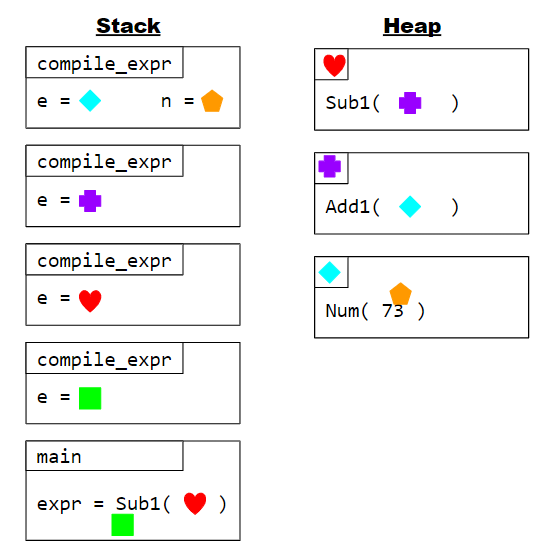
\includegraphics[scale=0.7]{../assets/memory_diagram.png}
        \end{center}
    \end{mdframed}
\end{mdframed}

\end{document}